\documentclass{article}

\usepackage{amsmath,amssymb,geometry,enumitem,graphicx,xepersian}

\setlength{\parindent}{0pt}
\setlength{\parskip}{3mm}

\newcounter{questionnumber}
\setcounter{questionnumber}{1}

\newcommand{\Q}{
\textbf{پرسش \thequestionnumber)}
\stepcounter{questionnumber}
}

\newcommand{\eqn}[1]{
\[\begin{split}
#1
\end{split}\]
}

\begin{document}
\Large
\begin{center}

به نام زیبایی

پایان ترم شبکه‌های مخابراتی

زمان: 120 دقیقه

\end{center}
\hrulefill
\large

\Q

توپولوژی زیر داده شده است:

\begin{figure}[h]
\centering
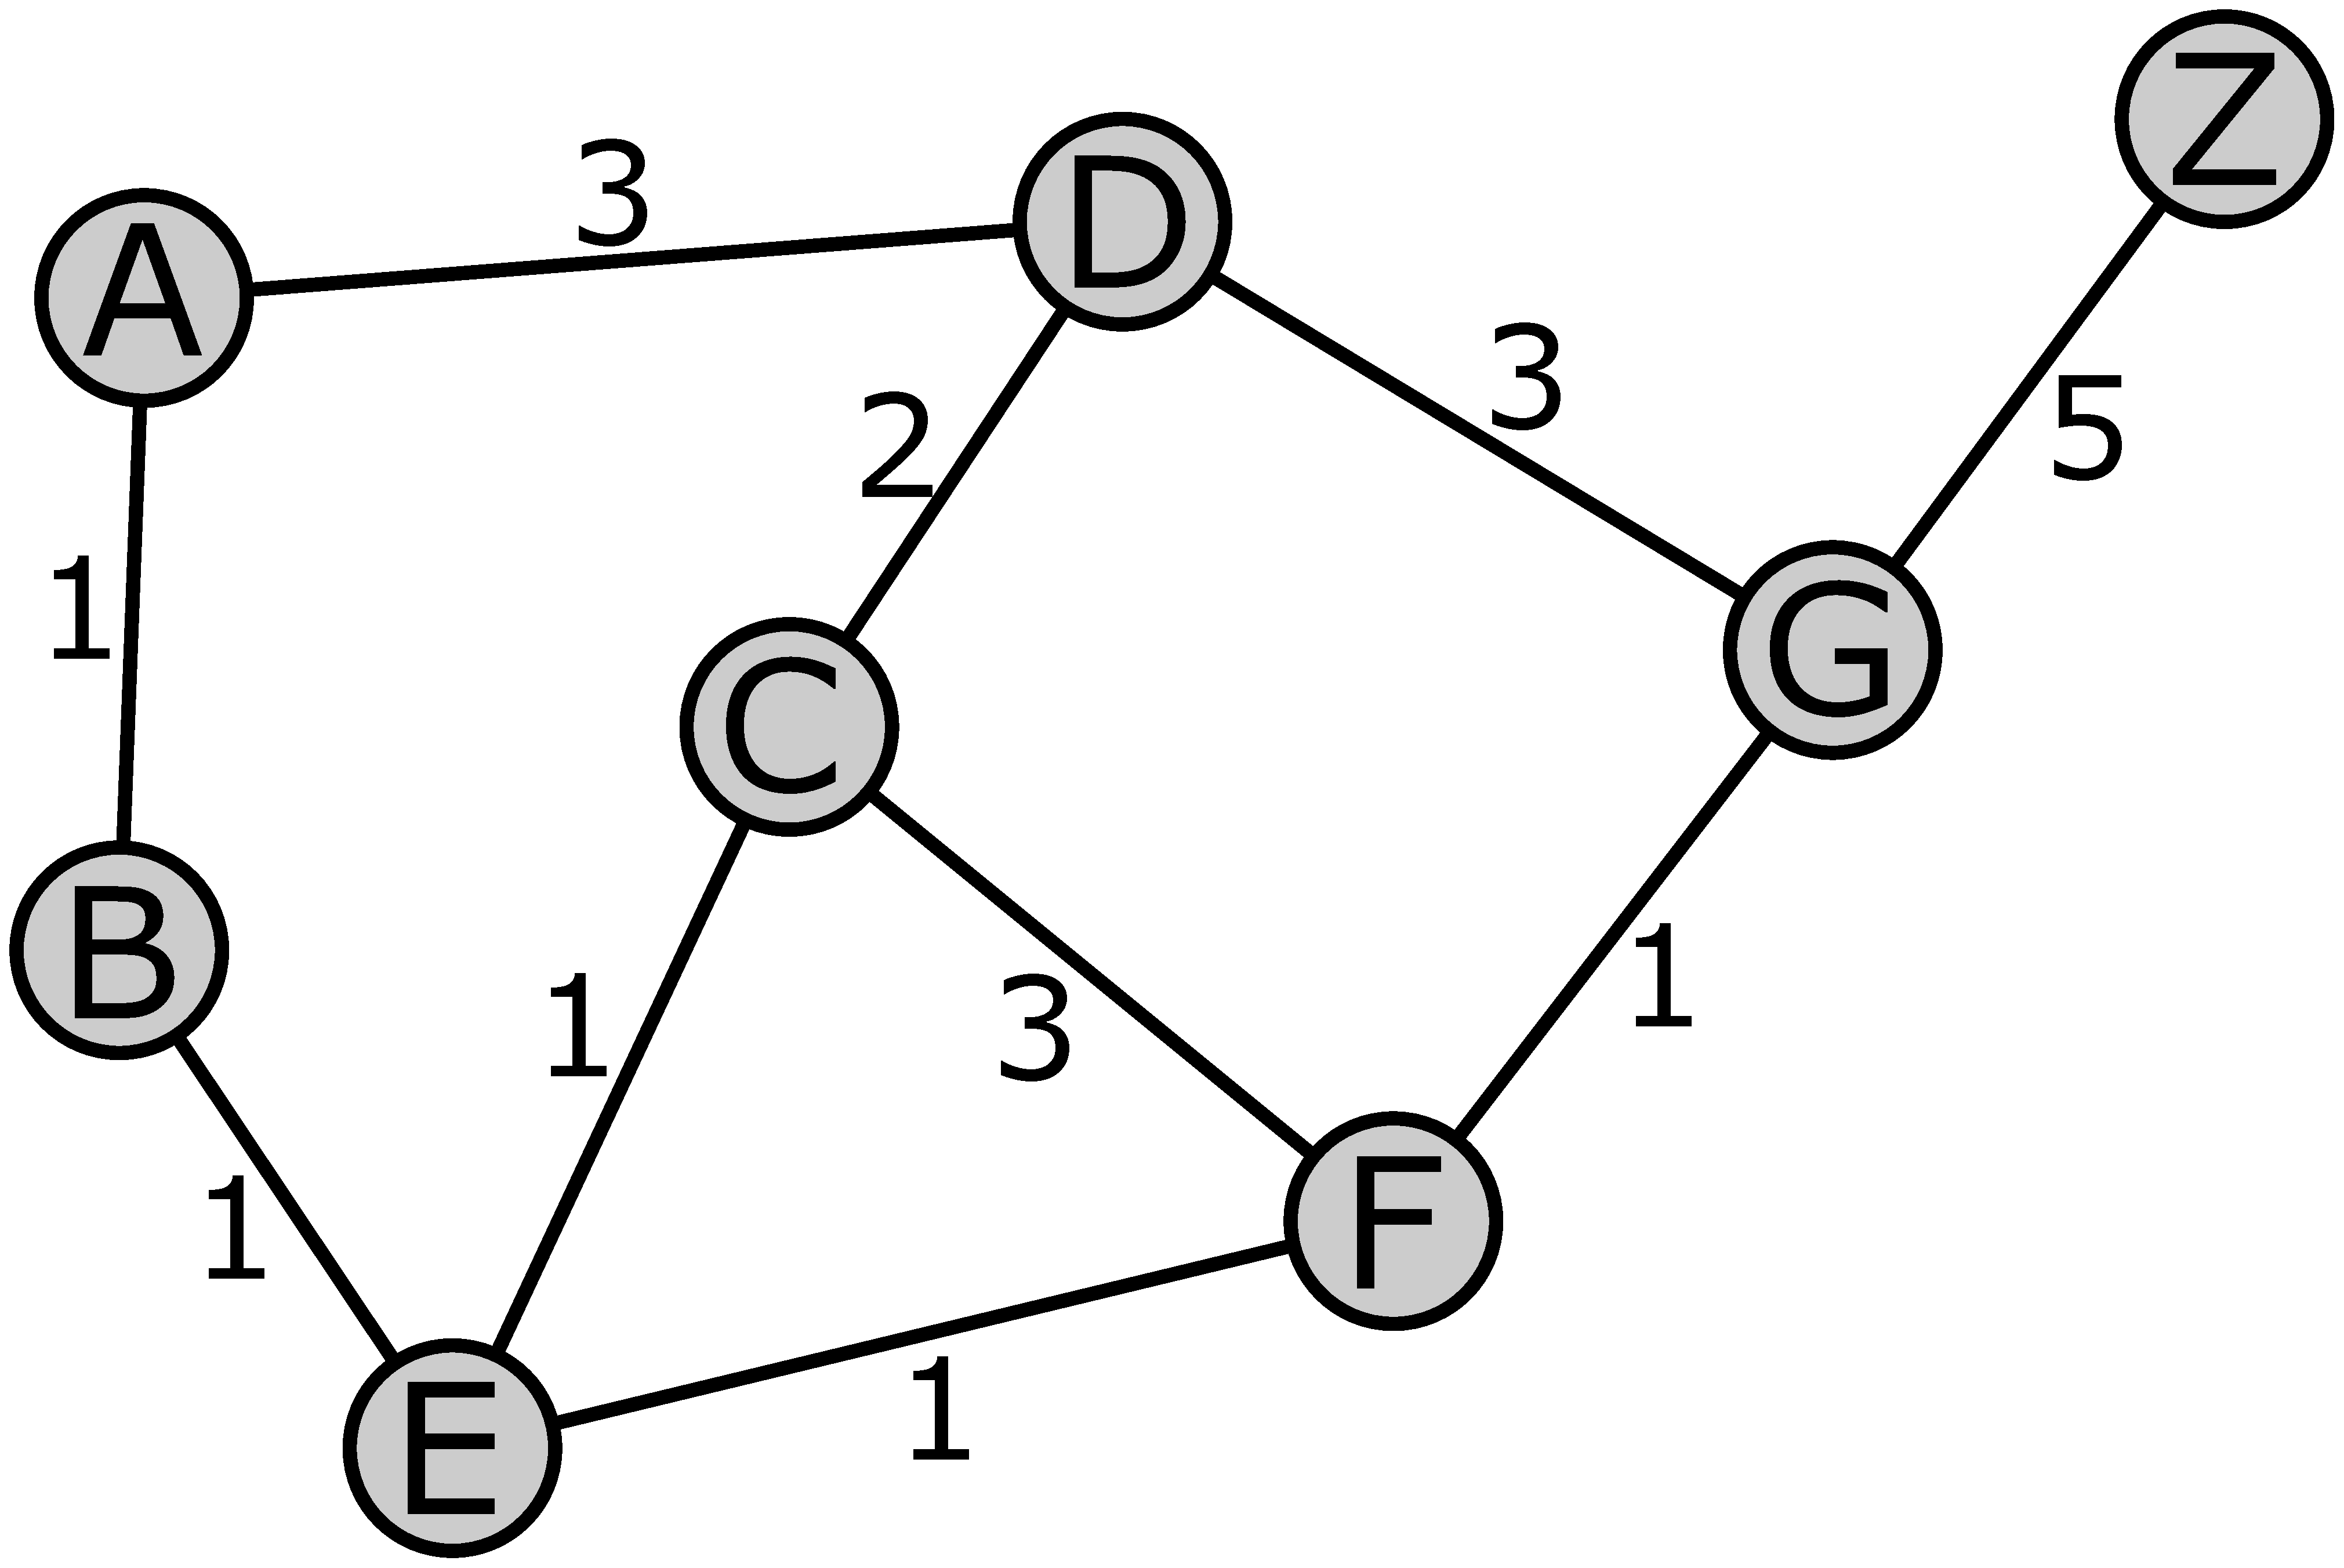
\includegraphics[width=80mm]{Q1_Final.eps}
\end{figure}

الف) با استفاده از الگوریتم دایکسترا، کوتاه ترین مسیر از \lr{A} تا \lr{Z} را بیابید.

ب) فرض کنید الگوریتم \lr{Bellman-Ford} برای محاسبه‌ی کوتاه ترین مسیر بین نودهای شبکه‌ی فوق استفاده شده باشد. اگر هزینه‌ی لینک \lr{EF} به 100 افزایش یابد، الگوریتم \lr{Bellman-Ford} برای تعیین مسیر بین \lr{C} و \lr{Z} به چه مشکلی بر می‌خورد؟ برای رفع این مشکل، راه حلی را پیشنهاد کنید و توضیح دهید این راه‌حل، چگونه مشکل بوجود آمده را رفع می‌کند.

\newpage

\Q

در شبکه‌ی زیر، فرض کنید نود \lr{A} بسته‌ای به حجم \lr{1Mbytes} را به سایر نودها \lr{Broadcast} کند. (احتمال آن که این بسته بر روی هر یک از لینکهای شبکه از یک نود به نود دیگر برسد، برابر $0.8$ است.)

\begin{figure}[h]
\centering
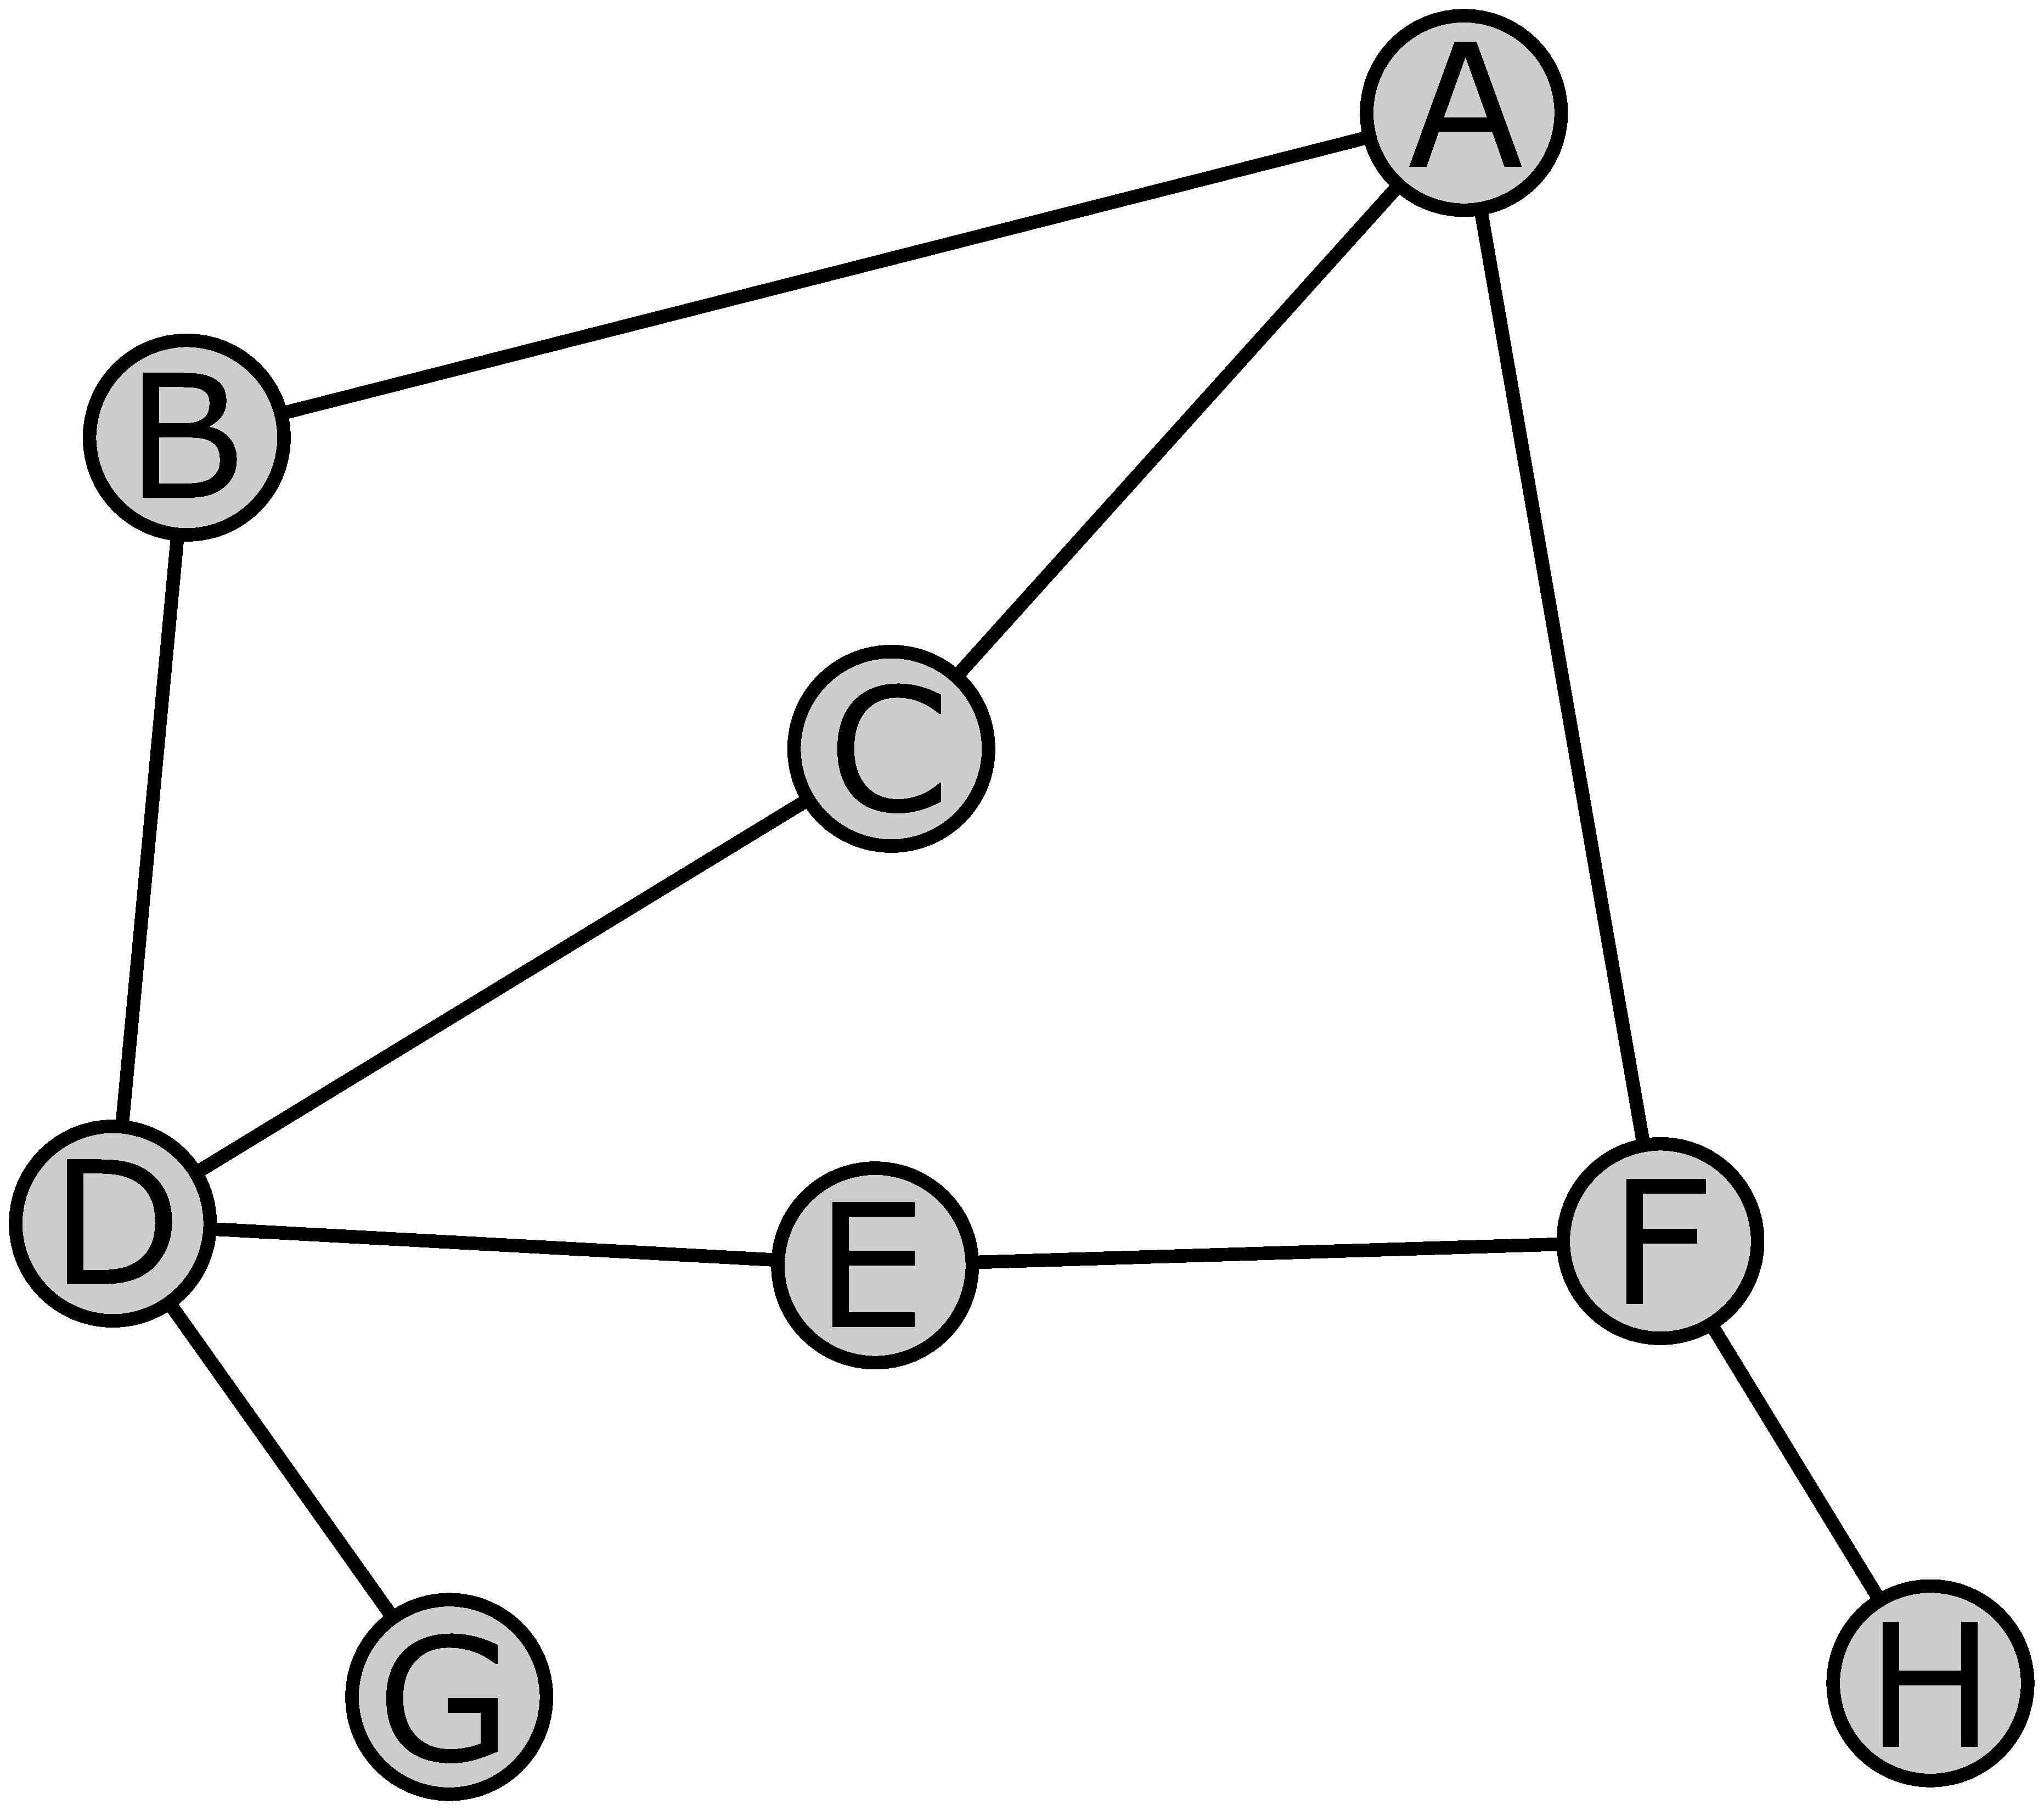
\includegraphics[width=60mm]{Q2_Final.eps}
\end{figure}

مجموع حجم بسته‌هایی که در شبکه مبادله می‌شوند (تا زمان دریافت موفق آمیز بسته توسط تمام نودها) چقدر است؟ اگر

الف)  هر نود به محض دریافت یک نسخه از این بسته، آن را روی تمام لینک‌های خود به سایر نودها ارسال کند؟

ب) یک بسته در هر نود زمانی پذیرفته شود که از لینکی که روی کوتاهترین مسیر بین این نود و نود \lr{A} قرار دارد دریافت شود؟ در صورت پذیرش، این بسته بر روی سایر لینکهای خروجی نود کپی می‌شود.

پ) از \lr{Minimum Spanning Tree} استفاده شده باشد؟ فرض کنید این درخت پیشتر محاسبه شده است (\lr{Minimum Spanning Tree}، خروجی الگوریتم دایکسترا از نود \lr{A} به سایر نودهاست).

(هزینه‌ی تمام لینک ها برابر 1 است.)

\newpage

\Q

دو کاربر جهت ارسال بسته های خود، از یک لینک مشترک و پروتکل \lr{Slotted Aloha} استفاده می‌کنند. مقادیر تایم اسلات، نرخ لینک و حجم بسته‌ها به ترتیب برابر
\lr{1msec}
،
\lr{100Mbps}
و
\lr{12.5Kbytes}
است. احتمال ارسال بسته (تکراری یا غیرتکراری) در هر تایم اسلات، برای کاربر 1 برابر
$
p_1
$
و برای کاربر 2 برابر
$
p_2
$
است. اگر هر دو کاربر در یک تایم اسلات مشخص، بسته‌های خود را ارسال کنند، هر دو بسته در لینک از بین می‌روند.

الف) نرخ مؤثر ارسال برای هر یک از کاربران چقدر است؟

ب) به ازای چه مقدار از $p_1$ و $p_2$، مجموع نرخ مؤثر ارسالی کاربران بیشینه می‌شود؟ اگر 
$
p_1=3p_2
$
باشد چطور؟

\newpage

\Q

آلیس می‌خواهد پیام m را رمزگذاری کرده و به باب منتقل کند. فرض کنید کلید های خصوصی و عمومی آلیس به ترتیب
$
K_A^-
$
و
$
K_A^+
$
و کلیدهای خصوصی و عمومی باب به ترتیب
$
K_B^-
$
و
$
K_B^+
$
باشند. در مراحل رمزنگاری زیر در سمت آلیس،
\begin{figure}[htbp]
\centering
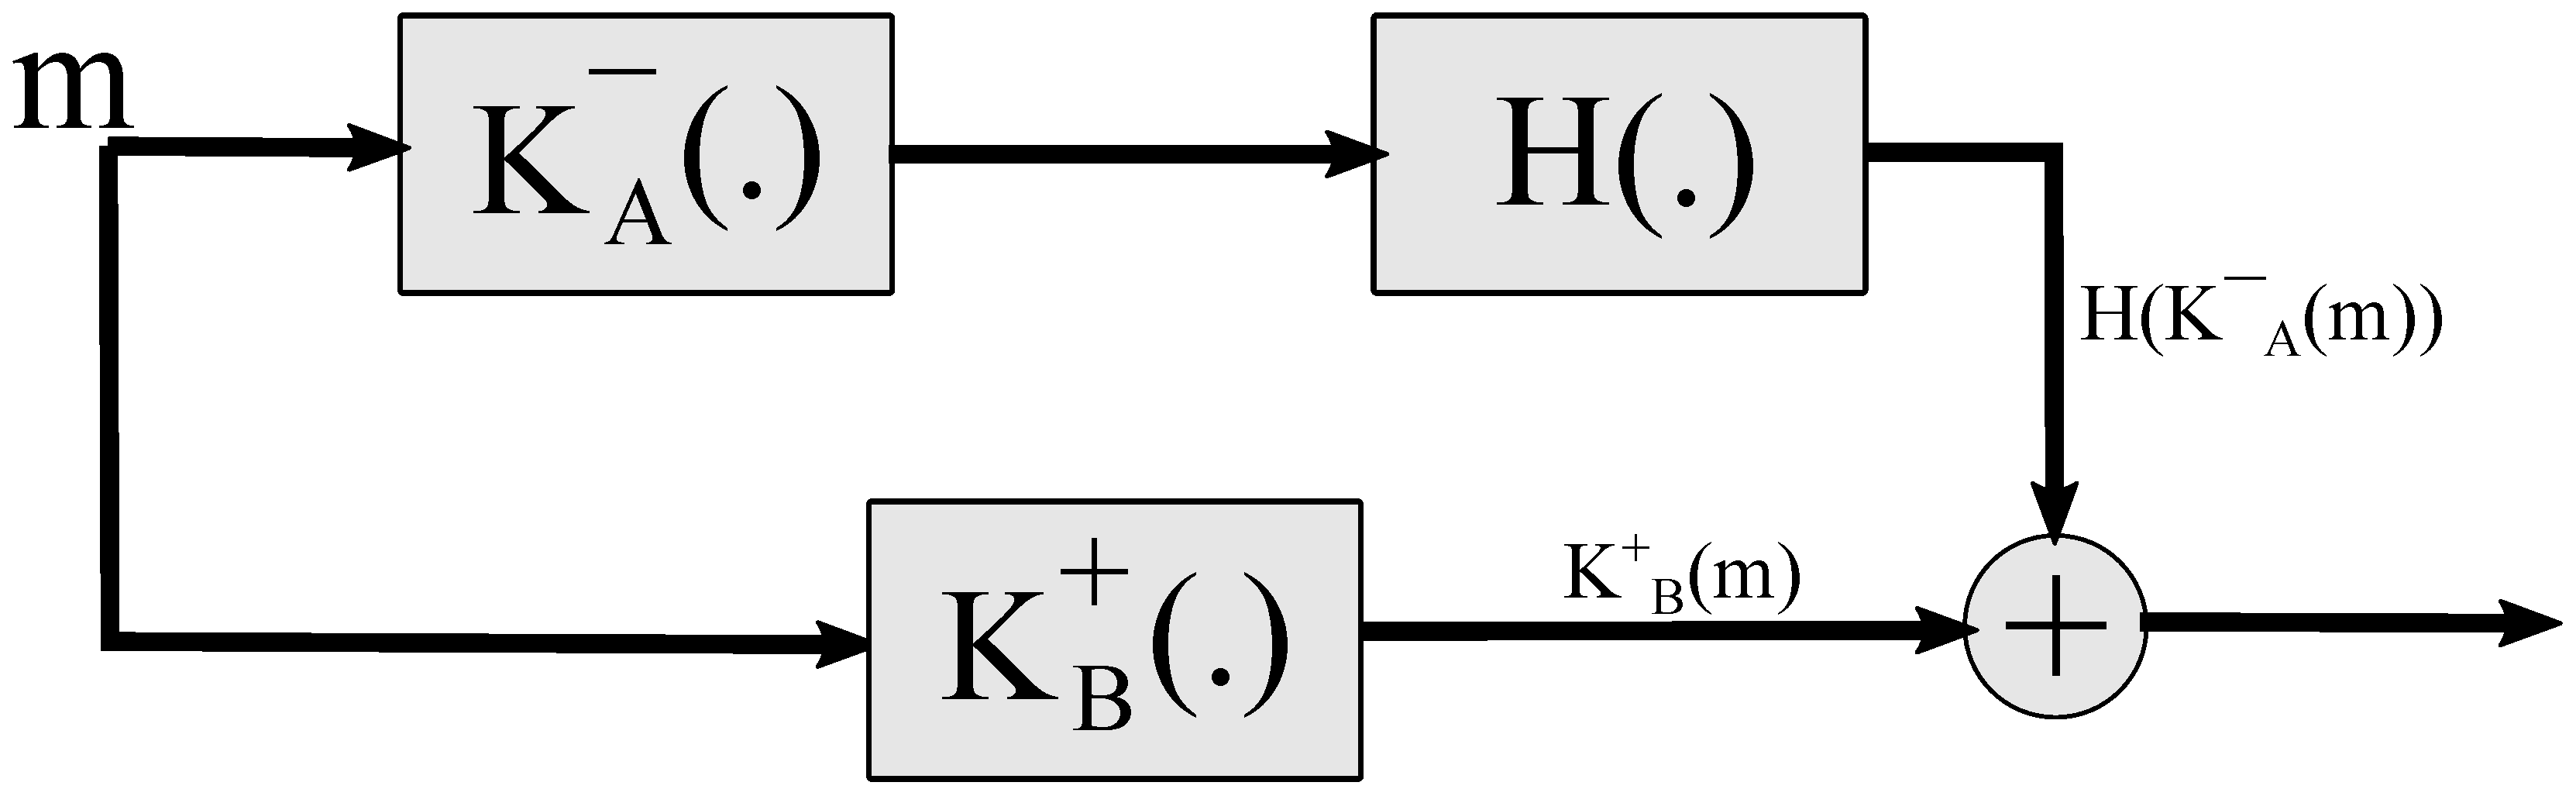
\includegraphics[width=100mm]{crypto.eps}
\end{figure}

الف) آیا تمام موارد محرمانگی پیام (\lr{Confidentiality})، اصالت پیام (\lr{Authentication}) و تمامیت پیام (\lr{Message Integrity}) حفظ شده اند؟ هر مورد را توضیح دهید.

ب) برای رفع مشکلهای مطرح شده در الف، چه راه حلی پیشنهاد می‌کنید؟

پ) پس از رفع مشکل قسمت ب، بلوک دیاگرام لازم را برای رمزگشایی پیام رسم کنید.

ت) باب برای تأیید اصالت کلید عمومی آلیس، چه سازوکاری را اتخاذ می‌کند؟ (\underline{جزئیات کامل})

ث) چنانچه آلیس بخواهد فایل 200 مگابایتی را به باب ارسال کند، چه ساختار بهتری برای رمزنگاری آلیس پیشنهاد می‌کنید؟ دلیل برتری ساختار پیشنهادی خود را بیان کنید.
\end{document}